\begin{figure}[tb]
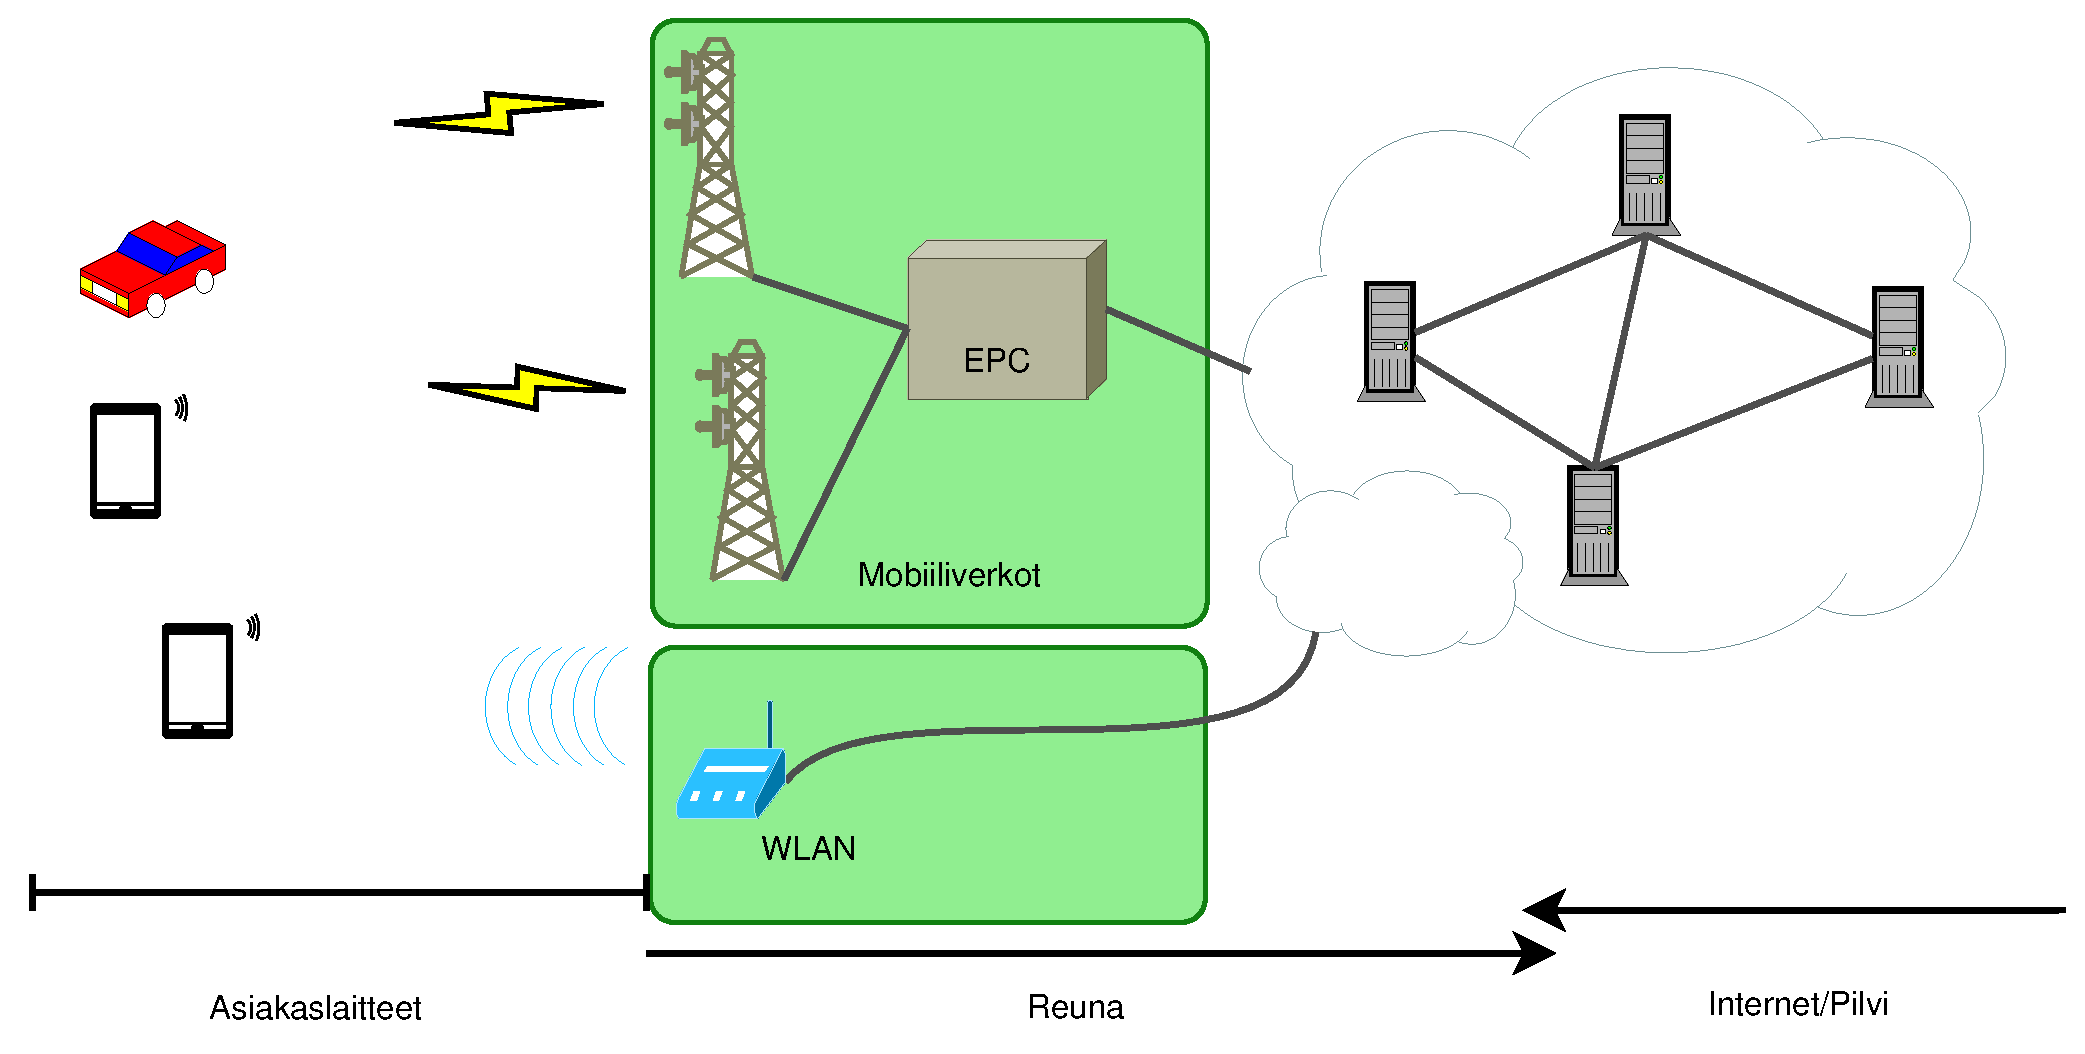
\includegraphics[width = \textwidth]{asiakasedgecloud.eps}
\caption{Asiakaslaitteiden, reunan ja pilven alueet} \label{fig:asiakasedgecloud}
\end{figure}

%Tähän voisi laittaa kuvan komponenttien asemmoitumisesta toisiinsa.
\subsubsection{Asiakaslaite}
Asiakaslaite (user equipment) on yleisnimitys reunan tai pilven palveluita kuluttavalla laitteelle.
Asiakaslaite -käsitettä ei ole rajattu mihinkään tiettyihin laitteisiin ja asiakaslaite voikin olla esimerkiksi älypuhelin, älylasit tai verkkoyhteydellä varustettu auto. 
Asiakaslaitteiden yhdistävänä tekijänä on siis jonkinlainen yhteys reuna- tai pilvipalveluihin. Yleisesti asiakaslaitteen käyttämä yhteys on tyypiltään langaton. 
Yksinkertaisuuden vuoksi tässä tutkielmassa asiakaslaitteen voi ajatella älypuhelimena, jollei toisin mainita.

Verkkohierarkian näkökulmasta asiakaslaitteet ovat lehtisolmuja. Tämä tarkoittaa että asiakaslaitteet toimivat ainoastaan palveluiden kuluttajina eivätkä siis tarjoa itse palveluita. Myöskään kulutettavien palveluiden tyypillä ei ole juurikaan merkitystä, kun asiaa käsitellään infrastruktuuri tai arkkitehtuuritasolla.

Konkreettinen esimerkki asiakaslaitteesta, joka hyödyntää reunapalvelua, voisi olla jokin ajoneuvo.
Ajoneuvolla on mobiiliyhteys reunapalveluun jonka tarkoitus on välittää tietoa liikenteestä muille ajoneuvoille. Esimerkiksi tilanteessa jossa edellä on ruuhkaa, voitaisiin muille lähistöllä oleville ajoneuvoille välittää tieto tästä, jolloin voidaan valita jokin toinen reitti määränpäähän.



\subsubsection{Reuna} \label{reunatoimijat}
Reuna koostuu useista toiminnallisista entiteeteistä, jotka voidaan jakaa sekä fyysisiin että loogisiin kokonaisuuksiin. 
Tässä kappaleessa lähdetään liikkeelle määrittelemällä reuna-alue, joka edustaa reunan toimialuetta sekä reunaa yleisenä käsitteenä.
Tämän jälkeen määritellään reunasolmu, joka on reunajärjestelmän keskeisin fyysinen rakennuspalanen.
Lopuksi esitellään pääasiassa ohjelmallisella tasolla ilmenevät toimijat reuna-alusta ja reunasovellus.


\paragraph{Reuna-alue} 
Tietyissä yhteyksissä reunalla viitataan alueeseen, joka alkaa asiakaslaitteen yhteyspisteestä. Se voi olla esimerkiksi WLAN-tukiasema tai mobiiliverkon tukiasema. Tästä ensimmäisestä yhteyspisteestä reuna-alue laajenee kohti runkoverkkoa ja pilveä.
Kuvassa \ref{fig:asiakasedgecloud} reuna on kuvattu alkavan mobiiliverkon tukiasemasta tai WLAN-tukiasemasta.
Joidenkin näkemyksien mukaan myös asiakaslaitteet luetaan osaksi reunaa, tällöin niihin viitataan termillä reuna laite (edge device) \cite{garcia}.
Tämän tutkielman puitteissa asiakaslaitteet luetaan omaksi osakseen reuna-alueen toisella laidalla.
Reunan laajuudelle ei siis ole yksiselitteistä määritelmää, vaan termiä usein sovelletaan käytettävän kontekstin mukaan siten, että reuna-alue rajautuu kontekstissa esiintyvien toimijoiden mukaan edellä mainitulle välille.
Esimerkiksi mobiiliverkon tukiasemien yhteyteen rakennettua reunajärjestelmää käsiteltäessä, reunalla tarkoitetaan ainoastaan reunajärjestelmän asiakaslaitteita palvelevien osien muodostamaa vyöhykettä. 
Kuten jo aiemmin mainittu, reunan keskeisenä etuna muihin palveluihin voidaan pitää reunapalveluiden ja asiakaslaitteen välisen viiveen vähäisyyttä.
Yleisenä nyrkkisääntönä reunalle voidaankin pitää verkkoyhteyksien viivettä suhteessa muuhun internettiin, koska reuna-alueella viiveiden tulisi siis olla muuta internettiä nopeampia. Toisin sanoen reunan palveluiden tulisi sijaita lähempänä kuin pilvessä sijaitsevien palveluiden.

\begin{figure}[tb]
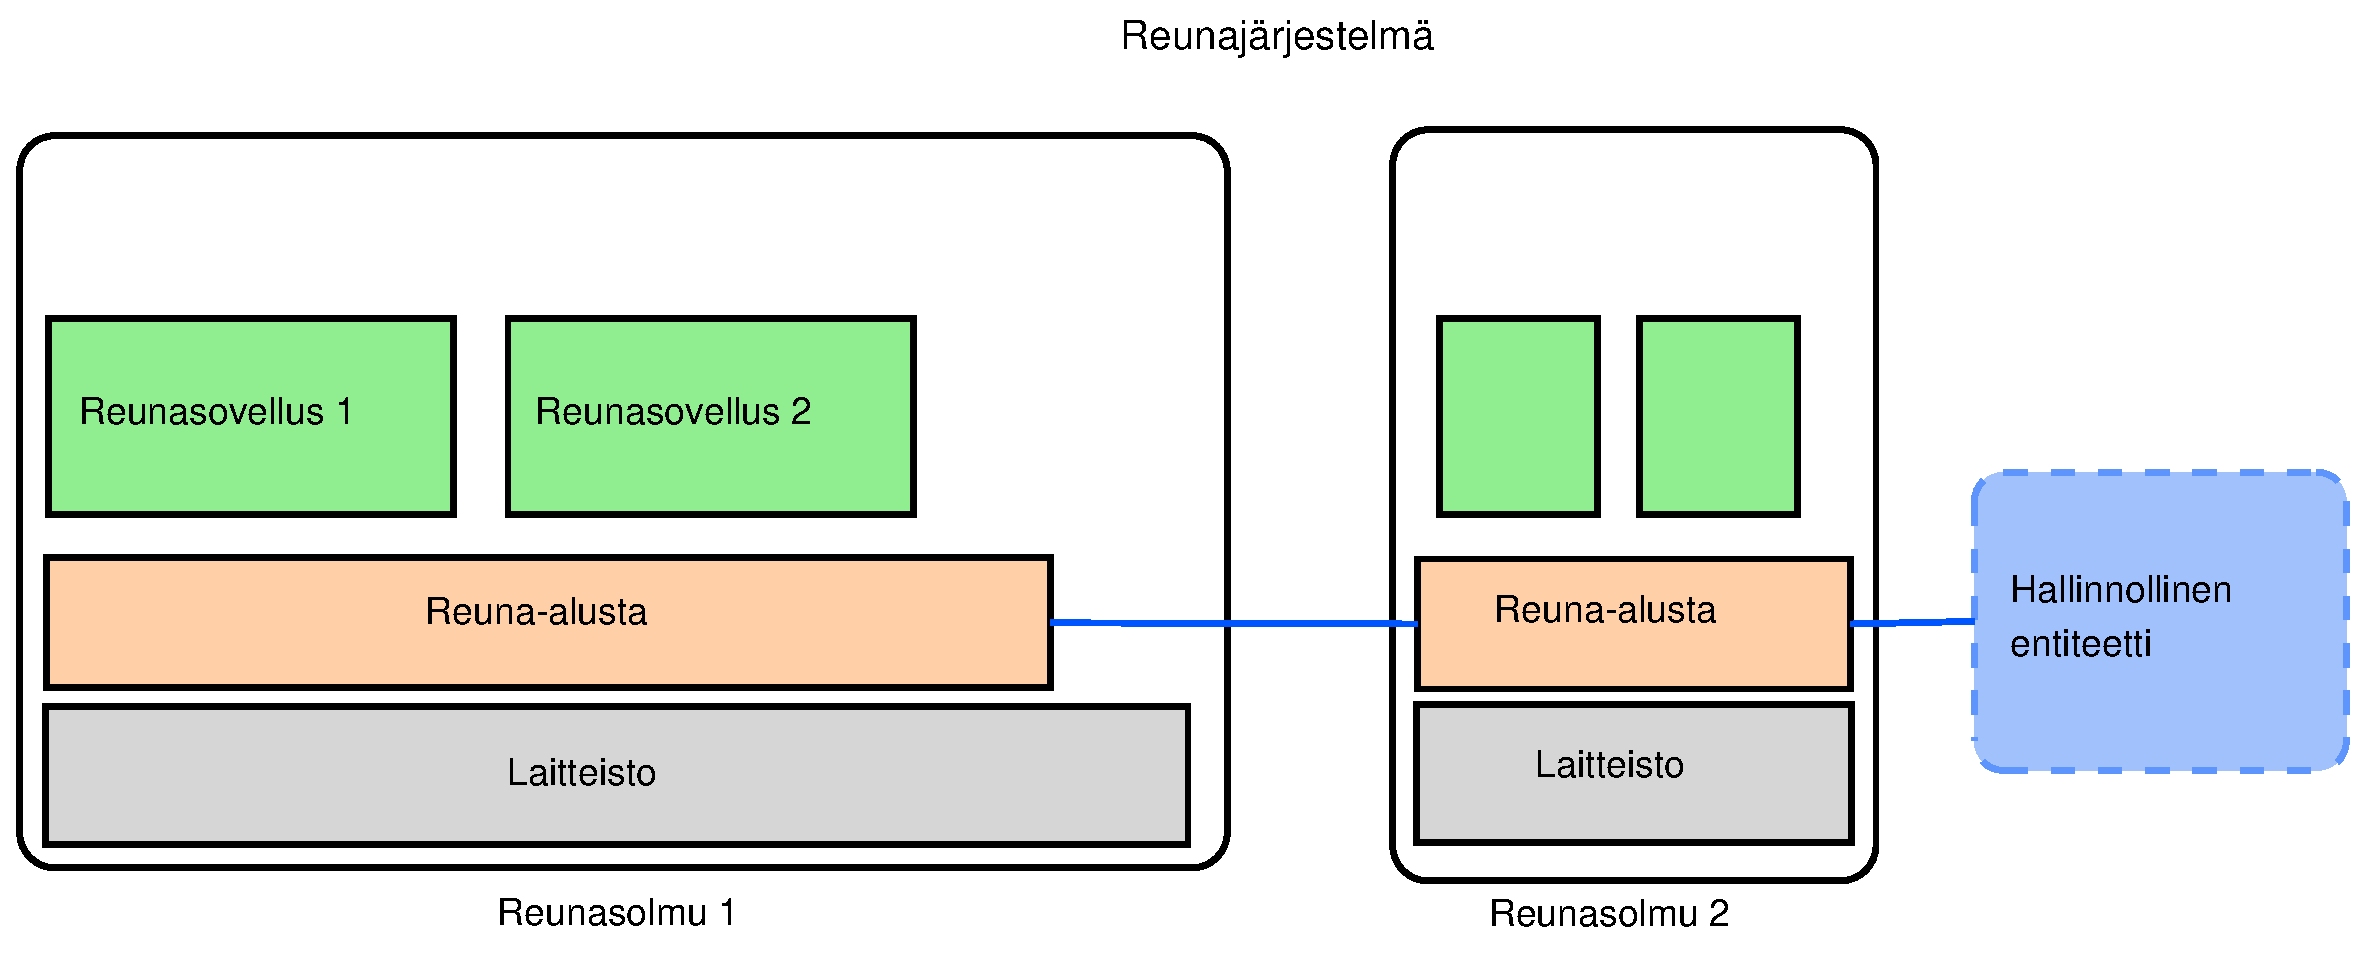
\includegraphics[width = \textwidth]{reunajarjestelma.eps}
\caption{Esimerkki reunajärjestelmän rakenteesta.} \label{fig:reunajarjestelma}
\end{figure}


\paragraph{Reunasolmu} 
Tämän tutkielman kontekstissa reunasolmulla (mobile edge host) tarkoitetaan yksittäistä reunalaskentaa tarjoavaa entiteettiä\cite{etsirefarch}.
Reunasolmu -termillä viitataan reunasolmun fyysiseen laitteiston ja reunasolmun toiminnalliseen kokonaisuuteen.
Reunasolmu sisältää reunasovelluksien suorittamiseen tarvittavat resurssit, jotka ovat pääasiassa tavallisia palvelinresursseja kuten laskenta, tallennustila ja verkkoyhteydet.
Reunasolmu voi koostua esimerkiksi mobiilitukiaseman ja palvelinlaitteiston muodostamasta kokonaisuudesta. 
Reunasolmun toiminnallinen kokonaisuus sisältää erinäisiä toimintoja, joiden tehtävänä on mahdollistaa reunasovelluksien suorittaminen.
Tällaisia ovat muun muassa tietoliikenteen reitittäminen ja virtualisointi-alustan tarjoaminen, sekä sen hallinnointi.
Kuvassa \ref{fig:reunajarjestelma} on esitetty esimerkki reunasolmun sisällä olevista entiteeteistä. 
Seuraavaksi käsiteltävä reuna-alusta kattaa osan reunasolmun toiminnoista.

Kuten aiemmin mainittu, reunajärjestelmä koostuu joukosta reunasolmuja, jotka ovat maantieteellisesti hajautettuja.
Reunasolmut siis eroavat toisistaan vähintään sijainnin perusteella, mutta voivat erota myös käytettävissä olevien resurssien osalta. Resurssien osalta reunasolmu voi olla mitä tahansa vähäisillä laskenta ja tallennus resursseilla varustetun WiFi-tukiaseman ja kokonaisen palvelinklusterin väliltä.
Reunasolmun sijaintiin vaikuttaa käytössä oleva reuna-arkkitehtuuri.
%Kuten juuri mainittu, reunasolmujen sijaintiin vaikuttaa käytettävä reuna-arkkitehtuuri.
Reunan rakennetta ja reunasolmujen sijaintia käsitellään tarkemmin luvussa \ref{rakenne}.

\paragraph{Reuna-alusta}
Reuna-alusta (Edge platform) on ohjelmistotason toimija. Se tarjoaa rajapinnan reunasovelluksien suorittamista varten\cite{etsirefarch}. Toisin sanoen se siis tarjoaa reunasovelluksille toimintaympäristön.
Reuna-alustan tehtävät eivät rajaudu ainoastaan yksittäiseen reunasolmuun, vaan sen lisäksi se hoitaa hallinnollisia tehtäviä kuten tietoliikenteen ohjausta. Lisäksi reuna-alustan tehtäviin voidaan lukea reunasovelluksia suorittaviin virtuaalikoneisiin liittyvät hallinnolliset toimet. Esimerkkinä reuna-alustan tehtävistä on kappaleessa \ref{livemigraatio} esiteltävä virtuaalikoneiden live migraatio reunasolmulta toiselle.
Reunasovelluksien lisäksi reuna-alusta voi itsessään tarjota palveluita, jotka eivät suoranaisesti ole reunasovelluksia vaan esimerkiksi nopea kommunikaatioväylä laitteelta-laitteelle (machine-to-machine), jota voi käyttää esimerkiksi ajoneuvojen väliseen kommunikointiin.
Koska reuna-alustan tehtäviin kuuluu hallinnolliset toimet, voidaan sen ajatella laajentuvan myös reunasolmun ulkopuolella sijaitseviin hallinnosta vastaaviin entiteetteihin.

\paragraph{Reunasovellus}
Reunasovelluksella (Edge application) tarkoitetaan yksittäistä reunasolmulla suoritettava ohjelmistoa \cite{etsirefarch}, jonka kuluttajana voi toimia asiakaslaite tai toinen reunasovellus. Reunasovellukset tarjoavat \textit{reunapalveluita}.
Reunasovellus ei ota kantaa millaista palvelua sillä tuotetaan.

Reunasovelluksen tuottama reunapalvelun tyyppiä säätelee pääasiassa reuna-alusta sekä reunalaskennan liiketoimintamalli. Teoriassa mahdollisuudet ovat siis samat kuin pilvessä.
Esimerkkejä reunasovelluksen tuottaman palvelun tyypeistä ovat yhteiskäyttöinen tai käyttäjäkohtainen.
Esimerkki käyttäjäkohtaisesta reunasovelluksesta voisi olla käyttäjäkohtainen virtuaalikone johon käyttäjä voi ottaa etäyhteyden. Esimerkkinä yhteiskäyttöisestä reunasovelluksesta voisi olla pelipalvelin, jota voivat käyttää reunasolmun toimipiirissä olevat pelaajat.

Reunalaskenta ja reunasovellus viittaavat yleensä lähes samaan asiaan, mutta eri konteksteissa. 
Reunasovellus on ohjelmallinen entiteetti, joka sijaitsee reunajärjestelmän sisällä.
Reunalaskenta puolestaan viittaa reunajärjestelmän palveluiden käyttämiseen.

\paragraph{Reunalaskennan tyypit}

Reunalaskennan tyyppejä ovat etälaskenta (offloading) ja asiakaslaitetta tukevat erilaiset reunapalvelut.
Arkkitehtuuritasolla reunalaskennan tyyppiin ei oteta juurikaan kantaa. 
Jotkin suunnittelupäätökset voivat kuitenkin vaikuttaa siihen millaisia reunalaskennan tyyppejä reunajärjestelmä lopulta tukee tai painottaa.
Etälaskennalla tarkoitetaan työyksiköiden (task) siirtämistä ulkoiselle laskentaa suorittavalle instanssille, joka palauttaa asiakaslaitteelle laskennan lopputuloksen. 
Reunajärjestelmässä suoritettava etälaskenta voidaan jakaa kahteen alakategoriaan: kokonaan reunalla suoritettaviin ja osittain reunalla suoritettaviin sovelluksiin\cite{mach17mobile}.
Kokonaan reunalla suoritettava laskenta on tyypiltään sellaista, että sitä ei voi jakaa useamman instanssin suoritettavaksi.
Tällöin vaihtoehdoksi jää suorittaa laskenta kokonaan paikallisesti tai siirtää se reunasolmulle suoritettavaksi.
Osittainen etälaskenta on vaihtoehto sovelluksille, jotka on mahdollista pilkkoa suoritettaviin työyksikköihin. 
Sovelluksen työyksiköt jakautuvat usein niihin jotka on mahdollista siirtää reunalle suoritettavaksi, sekä niihin joita ei ole mahdollista siirtää. 
Esimerkiksi valokuvan ottaminen on työyksikkö, jota ei ole mahdollista tehdä muuten kuin paikallisesti asiakaslaitteella \cite{mach17mobile}.
Päätös etälaskennan tekemistä on riippuvainen laskennan tavoitteesta. 
Tavoitteina voi olla esimerkiksi asiakaslaitteen virransäästön maksimointia tai laskennan suorituksen keston minimointia.
Reunapalvelu voi olla tyypiltään asiakaslaitteella suoritettavan sovelluksen toimintaa tukeva palvelu. Sen voi ajatella esimerkiksi pelipalvelimeksi, joka suorittaa pelimekaniikan simuloinnin ja asiakaslaitteelle jää tehtäväksi ainoastaan pelitilan visuaalinen esittäminen.  



\subsubsection{Pilvi}
%pilven alk peräinen määritelmä
Armbrust et al. esittävät artikkelissaan määritelmän pilvelle \cite{armbrust2010view}. 
Pilvellä viitataan sekä pilvessä tuotettaviin palveluihin, että itse järjestelmään.
Järjestelmällä tarkoitetaan pilvi-alustaa, joka mahdollistaa palveluiden tuottamisen.
Artikkelin mukaan pilven tuottamisen yhtenä keskeisimpänä mahdollistajana on toiminut edullisille sijainneille rakennetut suuret palvelinsalit.
Toisin sanottuna pilvipalvelut tuotetaan palvelinsaleissa, jotka ovat keskitettyjä ja sijaitsevat kauempana asutuksesta. 

Keskeinen osa pilvi paradigmaa on myös tapa jolla palveluita tuotetaan.
Pilvialusta tarjoaa asiakkailleen mahdollisuuden skaalata palveluitaan näennäisesti äärettömyyksiin.
Tämän lisäksi aika, jossa käytössä olevien resurssien lisäys tai poisto voidaan tehdä, on huomattavasti lyhyempi verrattuna perinteiseen palvelinsaliin, jossa palvelun käyttäjä omistaisi itse palvelun tuottamiseen käytettävän laitteiston.
Tässä tutkielmassa pilvellä viitataan kuitenkin enemmänkin järjestelmän rakenteeseen ja sijaintiin, kuin palveluiden tuottamiseen käytettävään malliin.

Reunan ei ole tarkoitus korvata pilveä, vaan täydentää sitä. Myöskään pilven ja reunan välinen raja ei ole tarkka. Tässä tutkielmassa pilvellä tarkoitetaan suhteessa reunaa kauempana sijaitsevia palveluita. Pilvi ulottuu verkon ytimestä kohti asiakaslaitetta ja saattaa olla osittain päällekkäin reunan kanssa. Kuten aiemmin mainittu, reuna lähestyy verkon ydintä asiakaslaitteen suunnasta. 

Pilven ja reunan väliin on ehdotettu vielä yhtä toteutusparadigmaa – sumua (fog computing).
Sumun tavoitteet ovat samankaltaisia kuin reunan. Sumun tavoitteita ovat muun muassa pienet viiveet, maantieteellisesti hajautettu rakenne ja langattomien laitteiden palvelu \cite{bonomi2012fog}. Sumun on tarkoitus olla hieman kuten pilvi, mutta hajautetumpana ja pilveen verrattuna huomattavasti lähempänä käyttäjää. Reunaan verrattuna sumu on hieman kuin reuna, joka on viety kauemmaksi verkon reunasta.
Sumua ei käsitellä tämän enempää tässä tutkielmassa, vaan keskitymme lähempänä reunaa sijaitsevaan laskentaan.



%Asiakaskohtaiselle reunainstanssille ei ole mitään vakiintunutta nimeä.
%Cloudlet on yksi ehdotettu toteutustekniikka tällaiselle asiakaskohtaiselle reunalla sijaitsevalle virtuaali-instanssille \cite{satya09}.

\subsubsection{Mobiiliverkko}
\begin{figure}[tb]
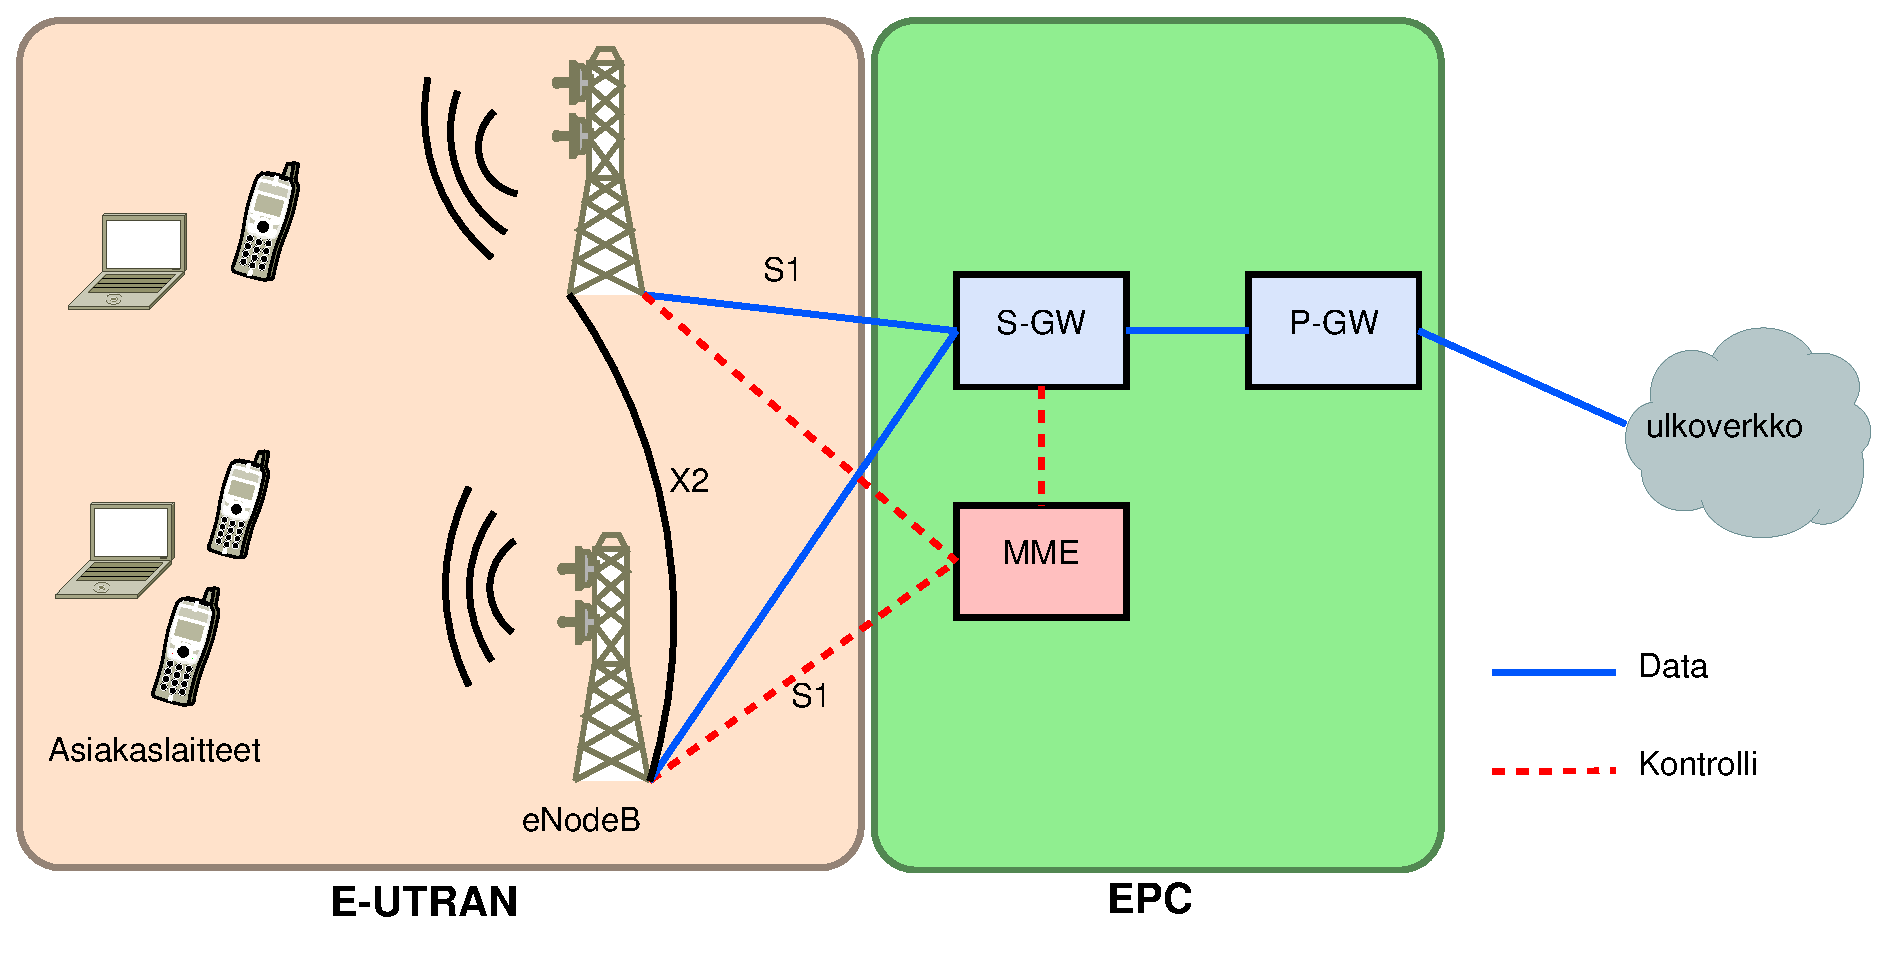
\includegraphics[width = \textwidth]{EPC.eps}
\caption{Yksinkertaistettu LTE-tyyppisen mobiiliverkon rakenne.} \label{fig:mobiarch}
\end{figure}

Tässä tutkielmassa käsiteltävät reuna-arkkitehtuurit sisältävät yhdistävänä tekijänä tavoitteen toimia mobiiliverkon yhteydessä. 
Täten reuna-arkkitehtuurien suunnittelupäätöksiä tarkasteltaessa on tarpeen ymmärtää mobiiliverkon osat yleisellä tasolla.
Yksinkertaisuuden vuoksi tämän tutkielman puitteissa mobiiliverkoksi oletetaan LTE:n mukainen arkkitehtuuri, joka koostuu E-UTRAN tyyppisestä radioverkosta ja EPC tyyppisestä runkoverkosta.
Seuraavaksi käydään läpi mobiiliverkon arkkitehtuurin tämän tutkielman kannalta merkitykselliset toimijat ja toiminnot.

Korkealla tasolla tarkasteltuna mobiiliverkko koostuu kahdesta osiosta: radioverkosta ja runkoverkosta. 3GPP kehittämässä LTE (Long Term Evolution) standardissa radioverkon sisältävä osuus on nimeltään E-UTRAN (Evolved UMTS Terrestrial Radio Access Network) ja runkoverkon osuus on nimeltään EPC (Evolved Packet Core).
E-UTRAN ja EPC väliset yhteydet on kuvattu kuvassa \ref{fig:mobiarch}.

E-UTRAN tehtävänä on toimia rajapintana asiakaslaitteen ja EPC:n välillä. 
E-UTRAN sisältää verkon puolella pääasiallisena toimijana eNodeB (Evolved nodeB) tyyppisiä tukiasemia \cite{etsieutran}.
Tukiasemista on olemassa muutamia erilaisia variaatioita, mutta tässä tutkielmassa käsitellään ainoastaan perustapausta.
Tukiasema on asiakaslaitetta lähimpänä sijaitseva funktionaalinen verkon osa ja sen seurauksena se on houkutteleva kohde reunalaskennan ratkaisuille. Tietoliikenteen näkökulmasta tukiaseman voi ajatella \textit{reunan} viimeisenä etappina ennen asiakaslaitteita. 

ENodeB tarjoaa asiakaslaitteiden suuntaan radioyhteyden.
EPC:n suuntaan eNodeB:t ovat yhteydessä S1 rajapinnan avulla.
Lisäksi eNodeB:t voivat olla toisiinsa yhteydessä X2 rajapinnan kautta.
S1:stä käytetään eNodeB:n ja EPC:n väliseen kommunikointiin. Tämä sisältää sekä hallinnollisen viestinnän, että asiakkaan tietoliikenteen kuljettamisen.
X2 rajapintaa puolestaan käytetään tukiasemien väliseen kommunikointiin. 
ENodeB välisten X2 yhteyksien tavoitteena on nopeuttaa tukiasemien välistä kommunikaatiota, esimerkiksi handoverin yhteydessä tehtävää asiakaskontekstin siirtoa varten \cite{3gpplte}.
Handoverilla tarkoitetaan asiakaslaitteen radioyhteyden siirtoa toiselle tukiasemalle. Handover käsitellään tarkemmin kappaleessa \ref{livemigraatio}.

Mobiiliverkon runkona toimiva EPC koostuu useista loogisista komponenteista.
Tämä siis tarkoittaa että toiminnallisuudet voivat fyysisesti sijaita samassa laitteessa. 
Tässä tutkielmassa on tarpeen ymmärtää perusteet seuraavista alikomponentista: MME (Mobility Management Entity), S-GW (Serving Gateway) ja PDN GW (P-GW, Packet data network gateway) \cite{etsilte}.
\begin{itemize}
\item \textbf{MME} on EPC:n hallinnollinen entiteetti joka vastaa muun muassa asiakaslaitteen tunnistamisesta ja handoveriin liittyvistä toimista EPC:n sisällä. Toisin kuin S-GW ja P-GW, MME ei käsittele asiakaslaitteiden tietoliikennettä.
\item \textbf{S-GW} eli palveluyhdyskäytävä toimii asiakaslaitteen EPC:n sisäisenä kiintopisteenä.  S-GW reitittää asiakaslaitteen liikennettä P-GW:n ja E-UTRAN välillä.
\item \textbf{P-GW} eli pakettiverkon yhdyskäytävän tehtävänä on toimia asiakaslaitteen ja mobiiliverkon ulkopuolisten IP-verkkojen yhteyspisteenä.
\end{itemize}
\cite{3gppepc}

Mobiiliverkossa käytävä kommunikaatio voidaan jakaa kahteen kerrokseen: kontrollikerrokseen ja tietoliikennekerrokseen.
Kontrollikerroksella välitettävät viestit ovat tarkoitettu hallinnollisiin toimintoihin mobiiliverkon sisällä. 
Tietoliikennekerros välittää asiakkaan tietoliikennettä internetin ja asiakaslaitteen välillä.
Asiakkaan tietoliikenne kulkee tukiaseman ja P-GW:n välillä GTP-tunneloituna (GPRS Tunnelling Protocol) \cite{puente15seamless}. Tämä tarkoittaa että mobiiliverkon sisällä tietoliikennettä ei ohjata asiakaslaitteen tietoliikenteen tunnisteiden pohjalta. 


\subsection{Reuna-arkkitehtuuri}
%Määrittele mikä on reuna-arkkitehtuuri

%REUNA-ARKKITEHTUURI ON JOUKKO SUUNNITTELUPÄÄTÖKSIÄ!

Tässä tutkielmassa käsiteltävät arkkitehtuurit koostuvat oletusarkkitehtuurin (framework) tai suunnittelumallin (design model) tyylisistä arkkitehtuurikuvauksista. 
Oletusarkkitehtuuri jakaa järjestelmän jonkin tehtävän toteuttaviin kokonaisuuksiin, kuten komponentteihin ja moduuleihin \cite{ohark}. 
Suunnittelumallit puolestaan kuvaavat tarkemmin järjestelmän komponentteja sekä niiden toimintoja. Suunnittelumallit ovat kuitenkin ainoastaan osajoukko suunnittelupäätöksistä \cite{ohark2}, joten ne jättävät osan päätöksistä toteuttajalle. Lisäksi suunnittelumallit kuvaavat järjestelmää ainoastaan jollain tietyllä abstraktiotasolla ja koko järjestelmän kattavaan kuvaamiseen tarvittaisiin useita sisäkkäisiä ja hierarkkisia suunnittelumalleja. 
Tässä tutkielmassa käsiteltävät reuna-arkkitehtuurit ovat korkean tason luonnehdintoja järjestelmän ja sen osien toiminnasta, jossain tietyssä ympäristössä.
Myös ETSI:n MEC referenssiarkkitehtuuri \cite{etsirefarch} sisältää vaatimusmaisesti esitetyt tarvittavat toimet, mutta ei kuvaa niiden toteutusta.
Toisin sanoen tutkielmassa käsiteltävät arkkitehtuurit kattavat vain osajoukon kaikista järjestelmän toteuttamiseksi tarvittavista suunnittelupäätöksistä.
 
Reuna-arkkitehtuurissa toiminnalliset osat on jaettu loogisiin kokonaisuuksiin, eli tehtävien mukaan kasattuihin komponentteihin. Reuna-arkkitehtuurit asettavat rajoitteita myös toimintojen fyysiselle sijoittumiselle, jolloin osa toimijoista on jaoteltu fyysisiin komponentteihin. Joskin kappaleessa \ref{nfv} esiteltävä NFV tekee toimintojen fyysisestä sijoittumisesta dynaamisempaa ja vähemmän laitteistoon sidonnaista. 
%Oletusarkkitehtuuria voidaan hyödyntää varsinaista toteutettavaa järjestelmää suunniteltaessa ja sovellusaluemallit kuvaavat järjestelmän osia suhteessa myös reunajärjestelmää ympäröiviin toimijoihin.
Kappaleessa \ref{reunatoimijat} käsiteltyjen reunan keskeisten käsitteiden mukaan tässä tutkielmassa reuna-arkkitehtuurit keskittyvät reunasolmun ja reuna-alustan toiminnalliseen määrittelyyn. 
Tämän lisäksi reunajärjestelmää käsitellään alijärjestelmänä, eli osana suurempaa kokonaisjärjestelmää, joka koostuu muun muassa mobiiliverkosta.
Kuten jo aiemmin mainittiin reuna-arkkitehtuurit eivät ota kantaa reunasovelluksien toimintaan

%Tämän tutkielman puitteissa arkkitehtuurilla tarkoitetaan reuna-alustan ja reunasolmujen muodostamaa järjestelmää. Reuna-alustan toiminnallisuuksia voisi eritellä vielä tarkemmin, etenkin reunasovelluksien hallinnan osalta. Cloudlet on konkreettinen toteutus reuna-alustan reunasovelluksia hallinnoivasta osasta, mutta se ei kata kuin yhden reunasolmun kerrallaan. 
%Tämän lisäksi olemassa on reunasolmujen välisestä hallinnasta vastaava kerros, tosin tämä kerros voi olla ulkoistettu erillisille hallinnolliselle toimijalle, jolloin hallinnollinen osa reuna-alustasta on varsinaisten reunasolmujen ulkopuolella. 

%Reunasovelluksien toimintaa ei käsitellä tarkemmin. Taxonomy paperissa on hyvä jaottelu erilaisista sovelluksista. Tämä aihepiiri laajenee sovelluksien jakamiseen osittain reunalla suoritettaviin (offloading) tai mobiilisovelluksen suoritusta tukeviin sovelluksiin. 

